\documentclass[10pt,a4paper]{article}
\usepackage[utf8]{inputenc}
\usepackage[italian]{babel}
\usepackage{amsmath}
\usepackage{amsfonts}
\usepackage{amssymb}
\usepackage{graphicx}
\usepackage{fullpage}
\usepackage{hyperref}
\usepackage{graphicx}
\usepackage{caption}
\usepackage{subcaption}

\author{Michele Carignani, Alessandro Lenzi}
\title{Analisi aggregata per ore}
\begin{document}

\maketitle

\section{Generazione dei grafi orari}

Per prima cosa i dati sono stati aggregati per ora. I dati originali del dataset 
%todo sistemare dataset
\href{https://dandelion.eu/datagem/telecom-mi-to-mi/description/}{Telecommunications - MI to MI} sono nel formato:
\begin{verbatim}
timestamp \t SourceId \t DestId \t Stregth
\end{verbatim}
e sono stati suddivisi in 24 file (uno per ogni ora) e aggregati, per cui
ogni file contiene (al massimo\footnote{poichè certi nodi possono non avere chiamate in uscita
in una certa fascia oraria.}) un record per ogni nodo nel formato:
\begin{verbatim}
SourceId \t DestId:Strength [\t DestId:Strength]
\end{verbatim}

A questo punto i pesi sugli archi (sopra chiamati \verb!Strength!) sono stati riscalati rispetto alla somma
dei valori della stella uscente di un nodo, ottenendo la probabilità di transire dal nodo $i$ al 
nodo $j$, ovvero:
$$ sumStrength_i = \sum_{j \in FS(i)} Strength_{ij} $$
$$ probability_{ij} = \frac{Strength_{ij}}{sumStrength_i} $$

\section{Ricerca delle componenti fortemente connesse}

Per ricercare le componenti fortemente connesse (in seguito CFC) sono stati utilizzati sia diversiti tipi di taglio degli archi, sia diverse strategie di visita.

\subsection{Tagli}
Un taglio degli archi su un valore $x$ significa utilizzare per la visita solo gli archi con peso (ovvero valore di probabilità) maggiore o uguale a $x$. Sono stati eseguiti test sui valori 0.001, 0.005, 0.007, 0.009, 0.01, 0.05,
0.07, 0.08, 0.09 e 0.1.

Vedremo i risultati dei tagli 0.005 e 0.05.

\subsection{Strategie di visita}
\textbf{Le strategie di visita} utilizzate sono 5 e impiegano i dati del dataset 
\href{https://dandelion.eu/datagem/telecom-sms-call-internet-mi/description/}{"Telecommunications - SMS, Call, Internet - MI"}:
a partire dai record del formato
\begin{verbatim}
SquareID \t Timestamp \t .. ChiamateInUscita ..
\end{verbatim}
per ogni ora sono stati generati file con record
\begin{verbatim}
SquareID \t AggregatedCalls
\end{verbatim}
che permettono di capire quale sia il valore assoluto proporzionale a tutte le chiamate in uscita dallo square
$ID$ in una certa fascia oraria.
In questo modo è possibile iniziare la visita del grafo non da nodi ordinati lessicograficamente ma in ordine
(crescente o decrescente) di traffico in uscita.
Le strategie inoltre si differenziano per il modo di ordinare la stella uscente da un nodo.
Perciò le strategie definite sono:
\begin{itemize}
\item SCC1: visita il grafo in ordine crescente di traffico uscente,
selezionando prima gli archi con probabilità maggiore;
\item SCC2: visita i nodi per traffico decrescente e con archi selezionati per probabilità crescente;
\item SCC3: visita i nodi per traffico decrescente e gli archi per probabilità crescente;
\item SCC4: visita dei nodi per traffico crescente e archi per probabilità crescente;
\item Stable: Esegue la ricerca delle SCC usando lo stesso ordine per tutti i file. %% todo scelto come?
\end{itemize}
 
\section{Risultati}

\subsection{Statistiche}

In fig. \ref{img:probs} sono mostrate le statistiche sui pesi degli archi come probabilità.
\begin{figure}
 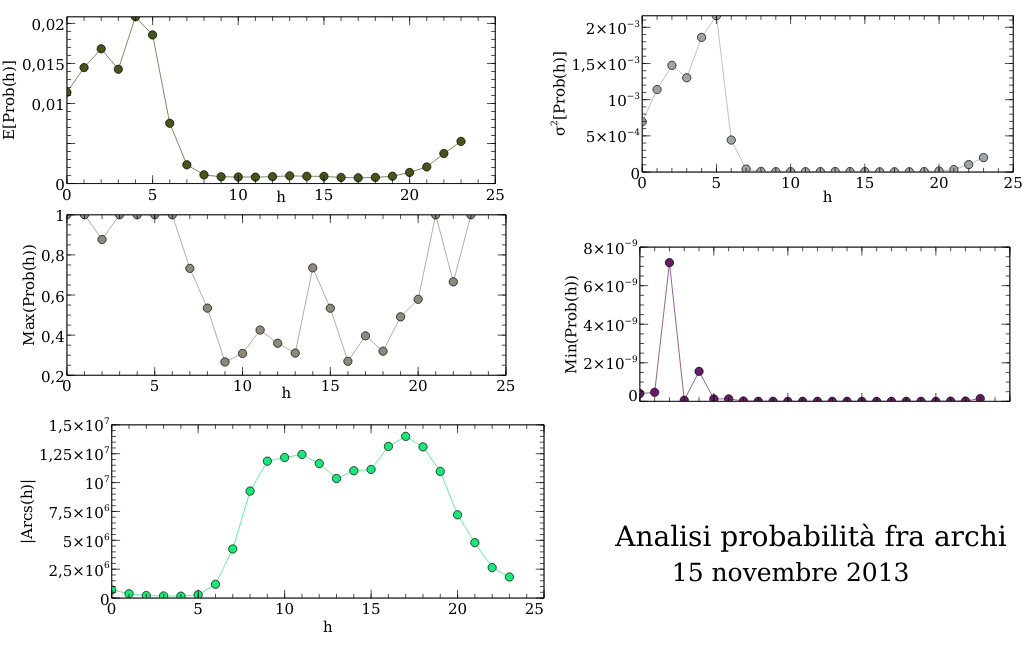
\includegraphics[scale=.6]{img/probs15nov.png}
 \caption{Statistiche sui pesi degli archi, 15 novembre. Sulle ascisse le fascie orarie, sulle ordinate le probabilità.}
 \label{img:probs}
\end{figure}

\subsection{Componenti Fortemente Connesse}

Le CFC sono state disegnate su mappe (utilizzando \verb!gnuplot!) assegnando una funzione $z$ alle celle di
coordinate $(x,y)$ così definita:
$$
z(x,y) =
\begin{cases}
0, & \text{se $(x,y)$ non appartiene ad alcuna CFC,} \\
10k, & \text{se $(x,y)$ appartiene alla k-esima CFC trovata.}
\end{cases}
$$

\subsubsection{SCC1, taglio 0.005}

\begin{figure}
\centering

\begin{subfigure}[b]{1\textwidth}
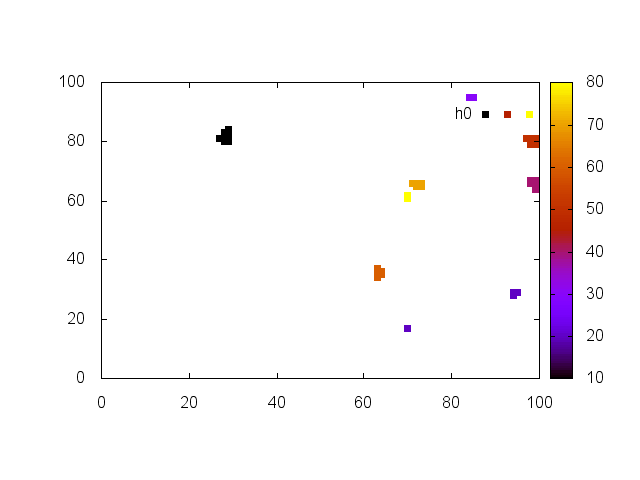
\includegraphics[scale=.3]{/home/miche/Desktop/plots/stampe/1/0.png}
\end{subfigure}

\begin{subfigure}[b]{1\textwidth}
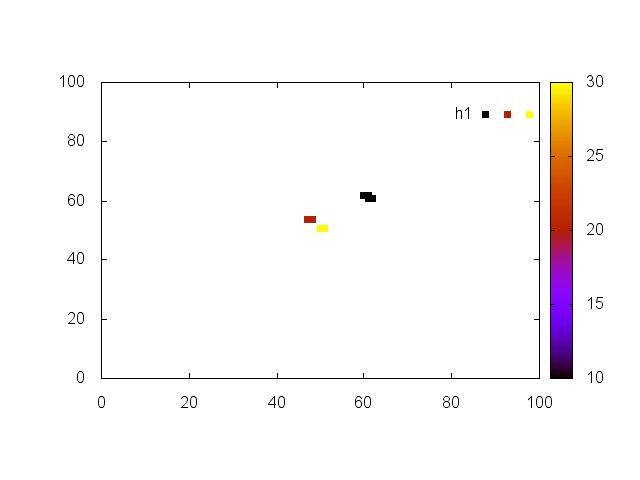
\includegraphics[scale=.3]{/home/miche/Desktop/plots/stampe/1/1.png}
\end{subfigure}
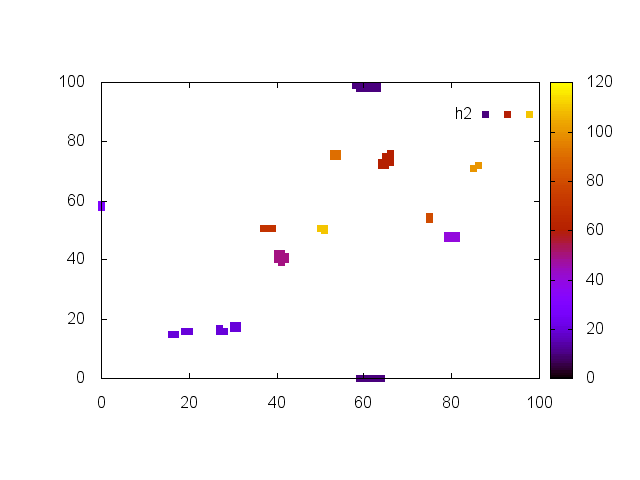
\includegraphics[scale=.3]{/home/miche/Desktop/plots/stampe/1/2.png}
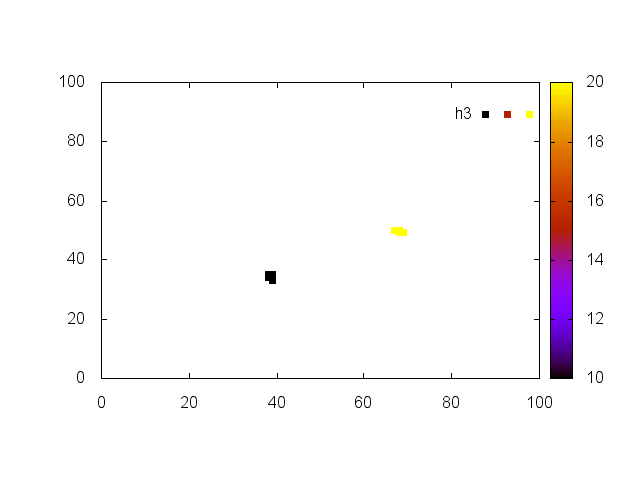
\includegraphics[scale=.3]{/home/miche/Desktop/plots/stampe/1/3.png}
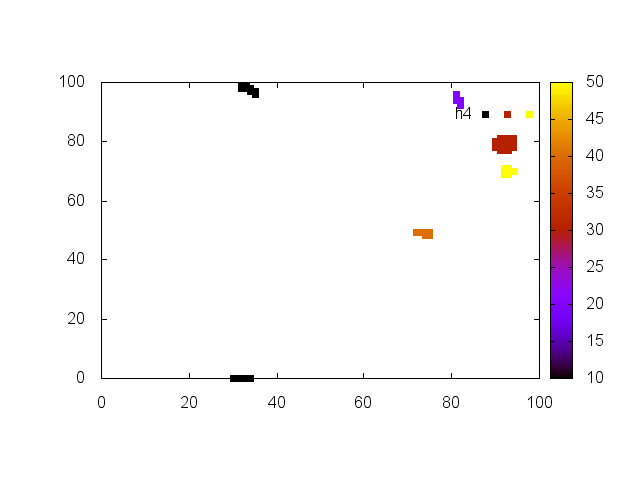
\includegraphics[scale=.3]{/home/miche/Desktop/plots/stampe/1/4.png}
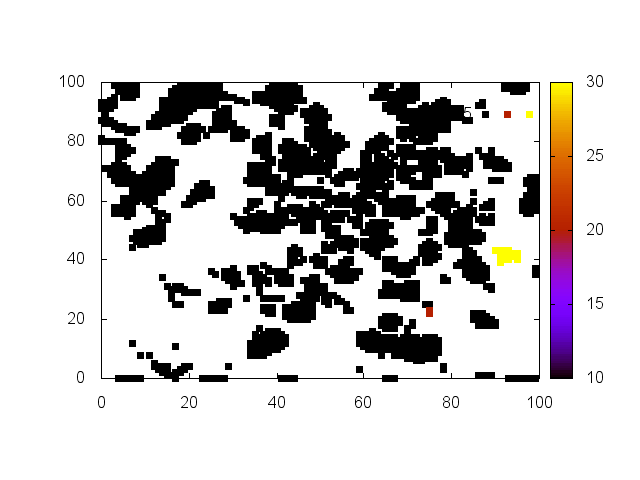
\includegraphics[scale=.3]{/home/miche/Desktop/plots/stampe/1/5.png}
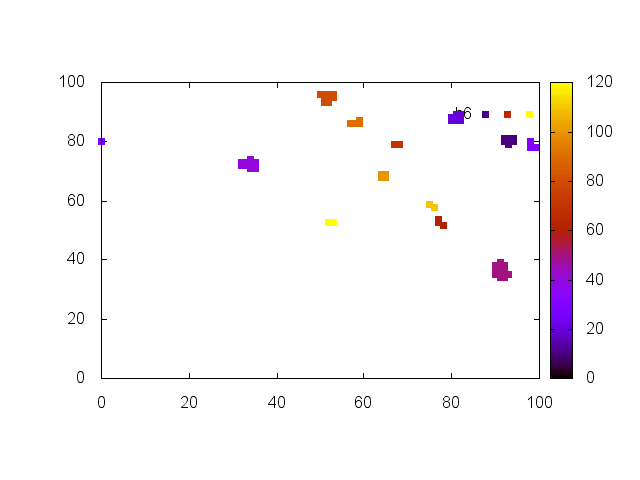
\includegraphics[scale=.3]{/home/miche/Desktop/plots/stampe/1/6.png}
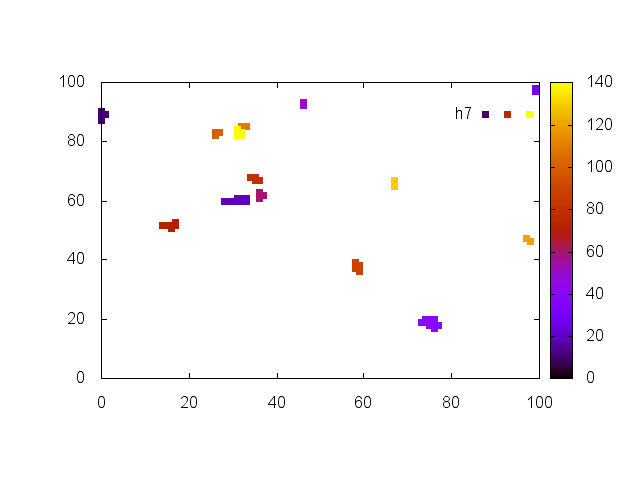
\includegraphics[scale=.3]{/home/miche/Desktop/plots/stampe/1/7.png}
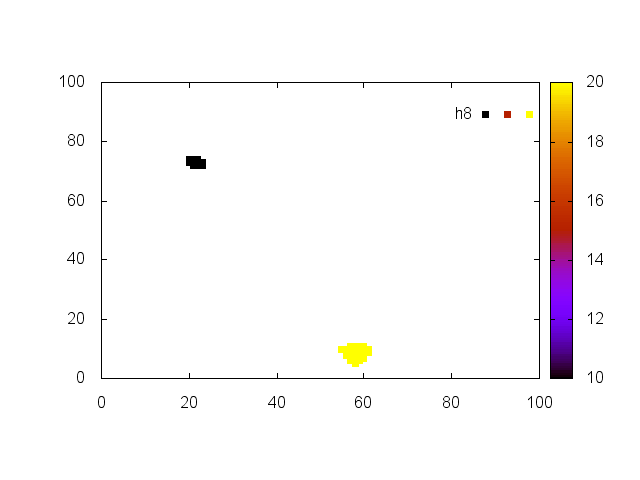
\includegraphics[scale=.3]{/home/miche/Desktop/plots/stampe/1/8.png}
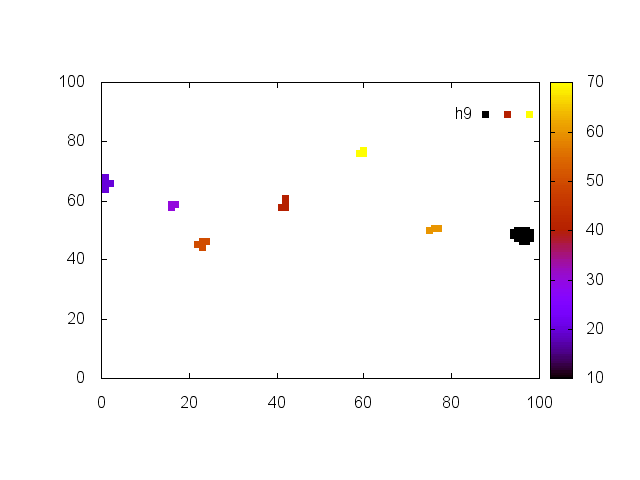
\includegraphics[scale=.3]{/home/miche/Desktop/plots/stampe/1/9.png}
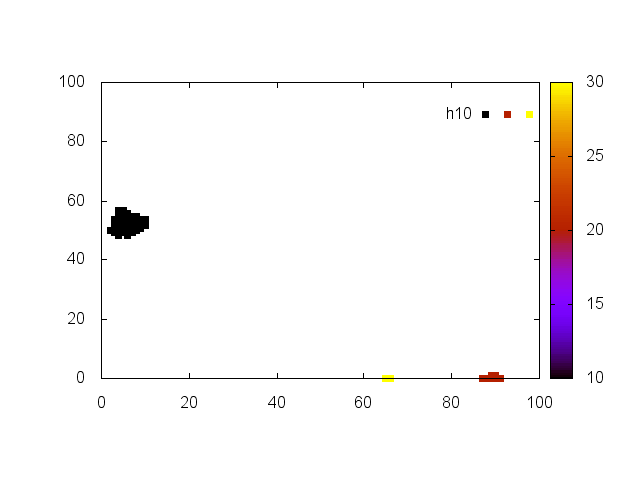
\includegraphics[scale=.3]{/home/miche/Desktop/plots/stampe/1/10.png}
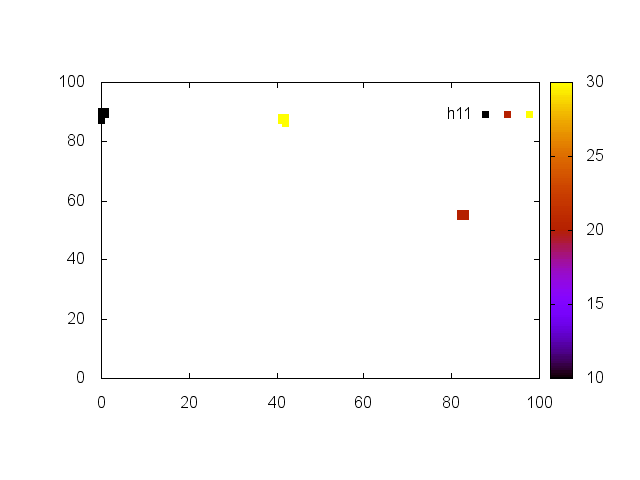
\includegraphics[scale=.3]{/home/miche/Desktop/plots/stampe/1/11.png}

\caption{SCC1, Taglio 0.005, h 0-11}
\end{figure}
\begin{figure}
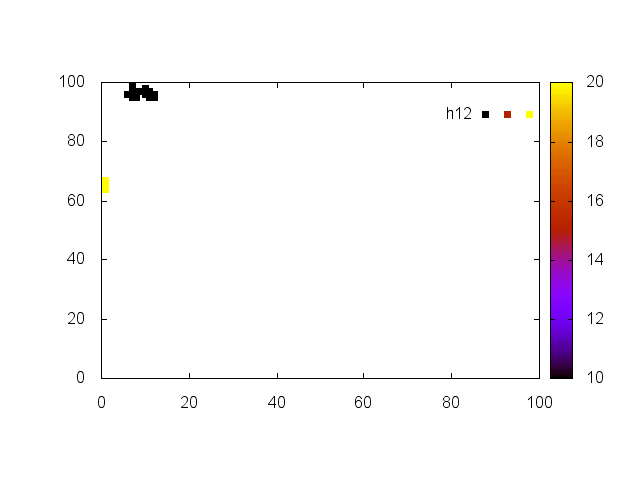
\includegraphics[scale=.3]{/home/miche/Desktop/plots/stampe/1/12.png}
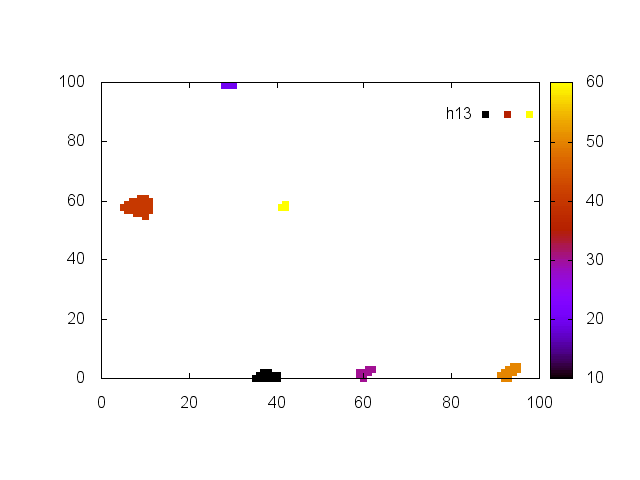
\includegraphics[scale=.3]{/home/miche/Desktop/plots/stampe/1/13.png}
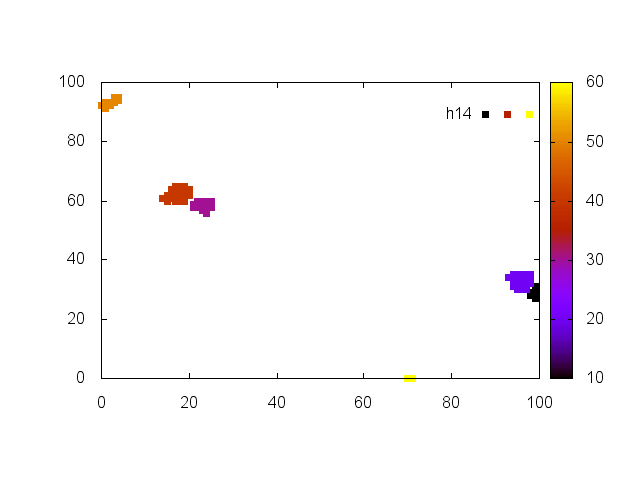
\includegraphics[scale=.3]{/home/miche/Desktop/plots/stampe/1/14.png}
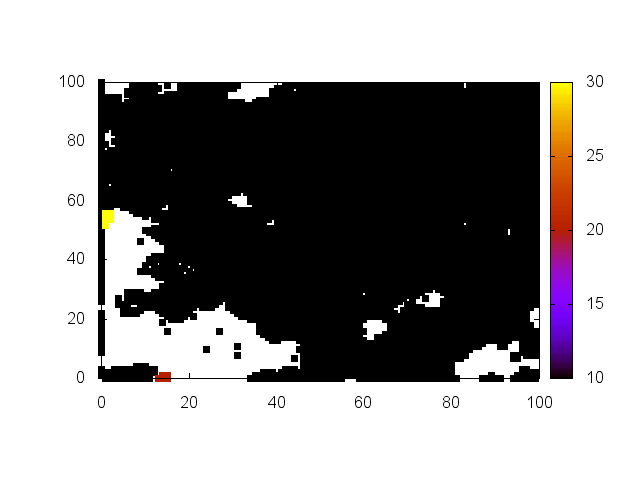
\includegraphics[scale=.3]{/home/miche/Desktop/plots/stampe/1/15.png}
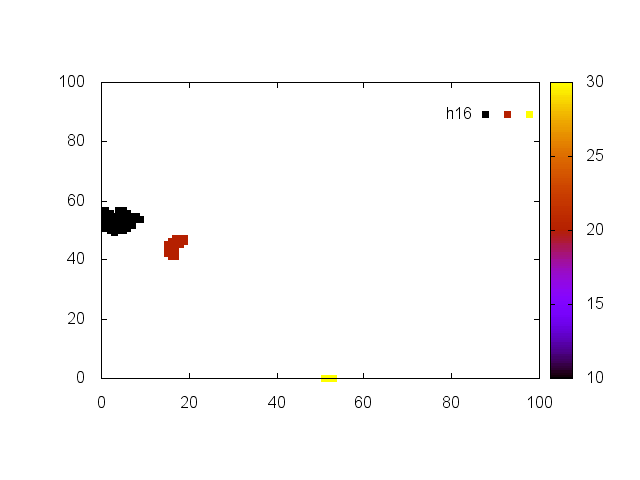
\includegraphics[scale=.3]{/home/miche/Desktop/plots/stampe/1/16.png}
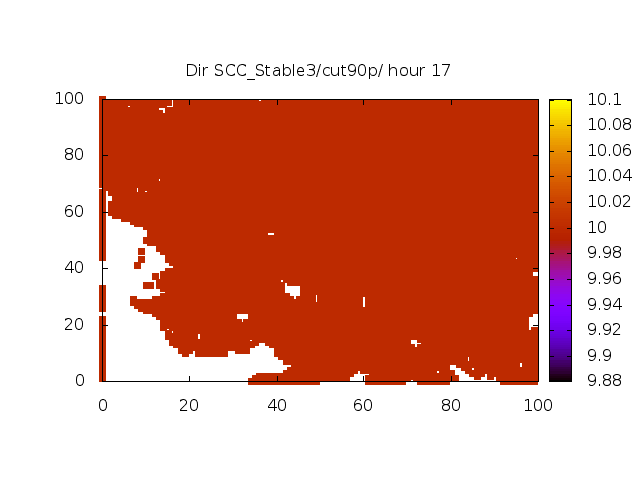
\includegraphics[scale=.3]{/home/miche/Desktop/plots/stampe/1/17.png}
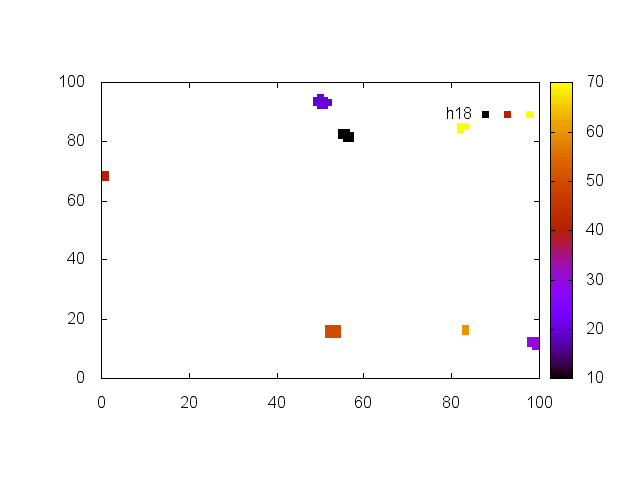
\includegraphics[scale=.3]{/home/miche/Desktop/plots/stampe/1/18.png}
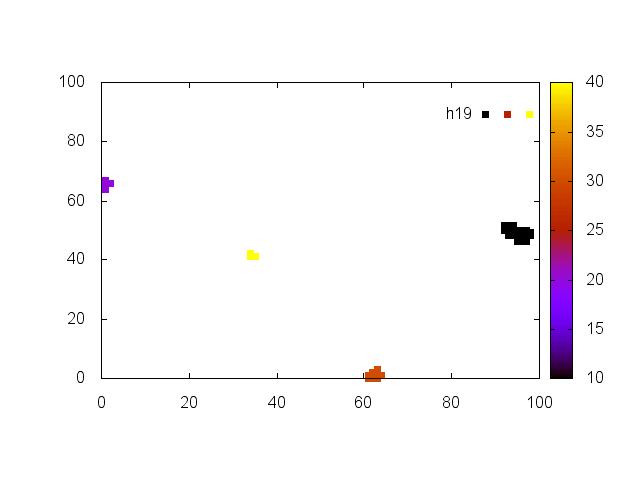
\includegraphics[scale=.3]{/home/miche/Desktop/plots/stampe/1/19.png}
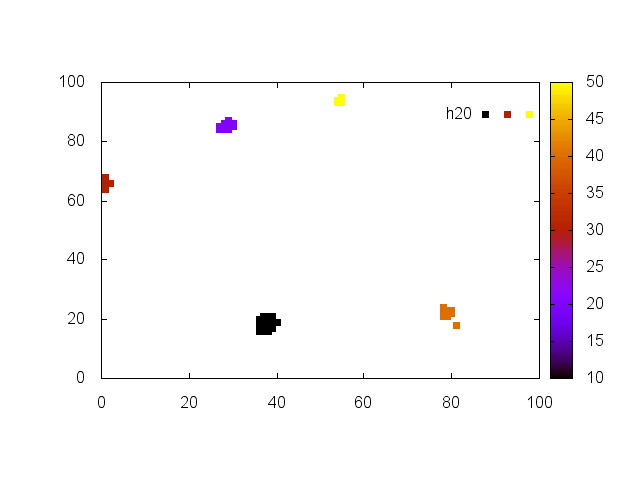
\includegraphics[scale=.3]{/home/miche/Desktop/plots/stampe/1/20.png}
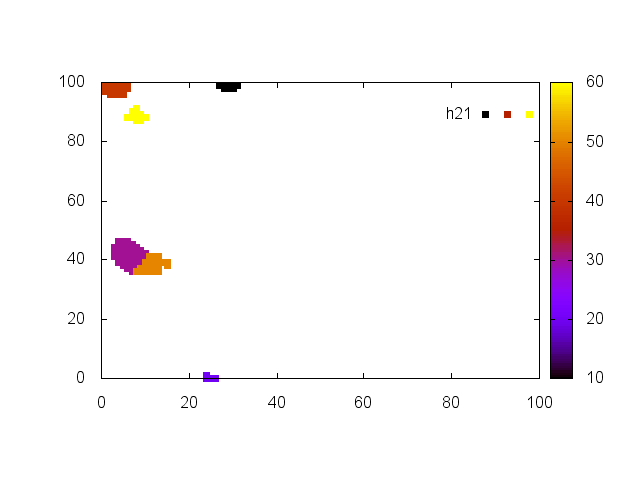
\includegraphics[scale=.3]{/home/miche/Desktop/plots/stampe/1/21.png}
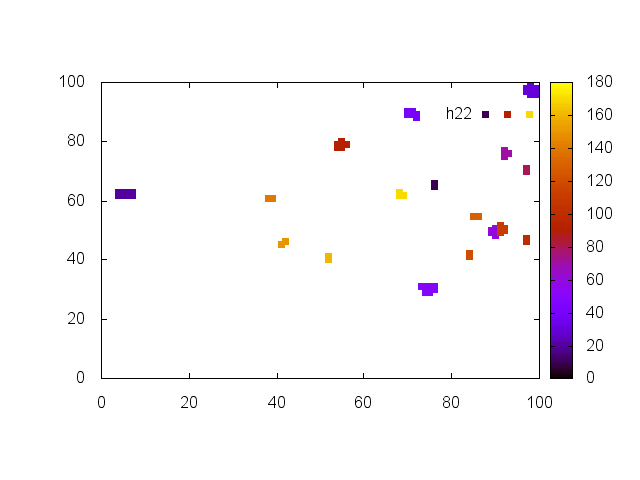
\includegraphics[scale=.3]{/home/miche/Desktop/plots/stampe/1/22.png}
\caption{SCC1, Taglio 0.005, h 12-22}
\end{figure}






\end{document}